\documentclass{article}

\usepackage{url} 

\usepackage[utf8]{inputenc}

\usepackage{pdfpages}
\usepackage{lastpage}
\usepackage{fancyhdr}
\usepackage{ngerman}
\usepackage{listings}

\usepackage{tabularx}
\usepackage{floatrow}
\usepackage[tableposition=top]{caption}
\floatsetup[table]{capposition=top}

\usepackage{amsmath, amssymb}

\usepackage[utf8]{inputenc}

\usepackage{xifthen}
\usepackage[numbib]{tocbibind}



\newcommand\twodigits[1]{%
   \ifnum#1<10 0#1\else #1\fi
}



\lhead{Spektralphotometer}
\rhead{20. November 2020\\T. Maier, J. Winkler}
%\cfoot{\twodigits{\thepage}~/ \pageref{LastPage}}
\cfoot{{\thepage}~/ \pageref{LastPage}}

\newcommand{\W}{\text{W}}
\newcommand{\V}{\text{V}}
\newcommand{\A}{\text{A}}


\newcommand{\mini}{\operatorname{min}}


\begin{document}

\parindent0cm

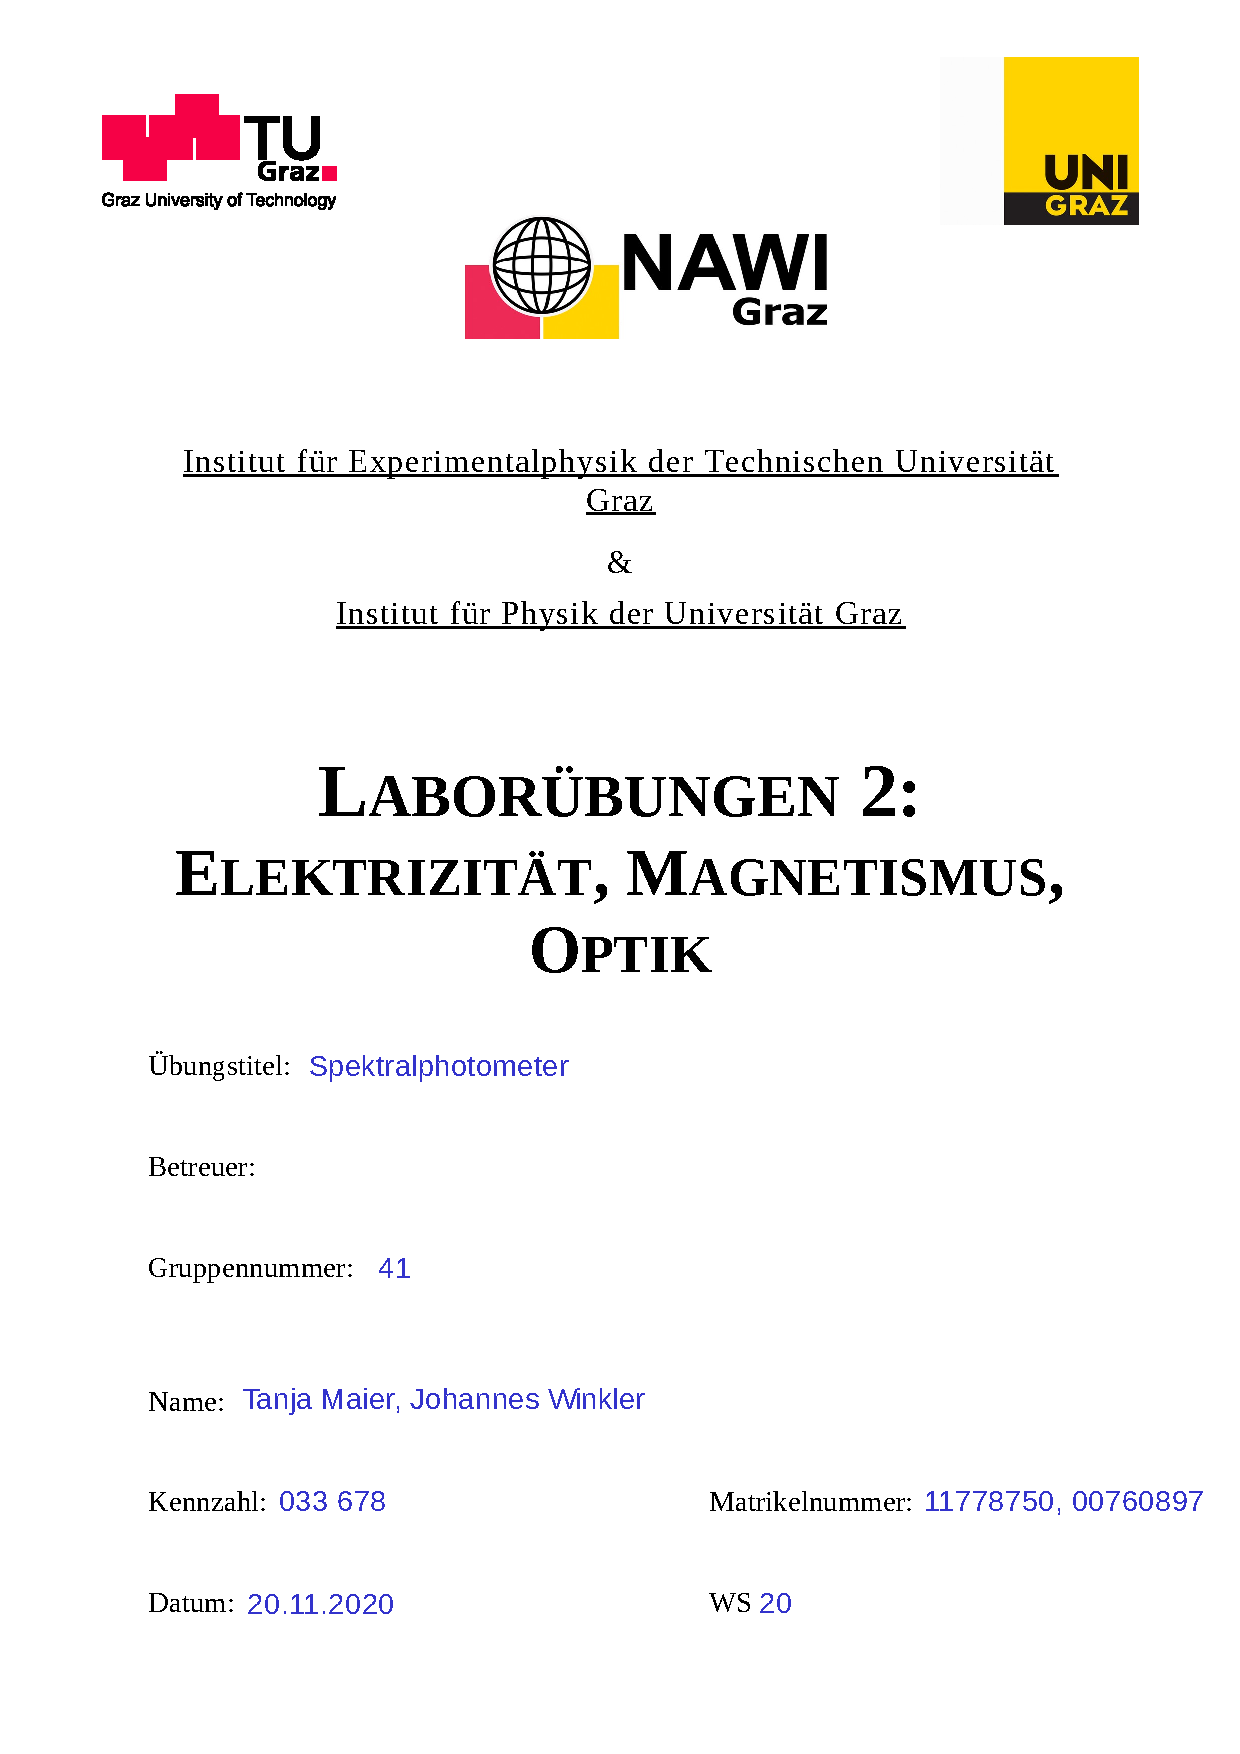
\includepdf{Deckblatt.pdf}


\pagestyle{fancy}

\tableofcontents
\newpage
\section{Aufgabenstellung}

\begin{enumerate}
\item Messen Sie mit dem Spektralphotometer die optische Transmission von Farbfiltern. Stellen Sie die Transmission und die (als logarithmisches Maß definierte) optische Extinktion als Funktion der Lichtwellenlänge dar. \item Zeigen Sie an zwei Farbfiltern die Additivität der Extinktion.
\item Bestimmen Sie die Stoffmengenkonzentration einer Methylenblaulösung. \item Diskutieren und erklären Sie anhand der gemessenen Spektren den Farbeindruck der jeweiligen Proben.
\item Messen Sie die Dicke einer Glasplatte durch Auswertung der Interferenzmaxima im Transmissionsspektrum
\end{enumerate}



\section{Voraussetzungen und Grundlagen}

\subsection{Transmission, Extinktion, Absorptionsquerschnitt}

Wenn Licht auf verschiedene Stoffe und Materialien scheint, kann es in unterschiedlichen Frequenzen oder Wellenlängen reflektiert, absorbiert und gestreut werden. Trifft Licht auf eine glatte Oberfläche oder einen homogenen Körper, so wird die Streuung Reflexion genannt. Beim Einfall auf eine teiltransparente Schicht ist das Verhältnis der transmittierten (als durch das Medium durchgelassenen) Intensität $I_T$ und der auf das Medium scheinende Lichtintensität $I_0$ gegeben durch
\begin{align}
T = \frac{I_T}{I_0}
\end{align}
wobei $T$ als Transmission bzw. Transmissionsgrad bezeichnet wird. Wichtig ist, dass $T < 1$ ist, da immer ein gewisser Teil des Lichts beim Kontakt mit dem Medium in eine andere Energieform (z.B. Wärme) umgewandelt (also absorbiert) oder einfach in andere Richtungen reflektiert (bzw. gestreut) wird.

Allerdings kann aus der Messung der transmittierten Intensität meist nicht auf jene Intensitätsanteile, die gestreut bzw. die absorbiert werden rückgeschlossen werden. Daher wird in der Spektroskopie oft das dekadisch logarithmische Maß der Lichtabschwächung (Extinktion) verwendet:

\begin{align}
E = -\log(T) = -\log\left(\frac{I_T}{I_0}\right) = \log\left(\frac{I_0}{I_T}\right)
\end{align}

Falls mehrere Extinktionsprozesse stattfinden, so können diese wegen der Gesetze für Logarithmen addiert werden. Außerdem können durch das logarithmische Maß Variationen von Lichtabschwächung über mehrere Größenordnungen übersichtlich dargestellt werden.

Die Lichtabschwächung bei einem homogenen Medium kann durch das Lambert-Beer'sche Gesetz beschrieben werden
\begin{align}
I_T(d) = I_0 \cdot \exp\left(-\alpha\cdot d\right)
\end{align}
wobei $d$ die Schichtdicke des Mediums und $\alpha$ der Extinktionskoeffizient ist.

Der Extinktionskoeffizient $\alpha$ hängt dabei vom molaren Extinktionskoeffizienten $\varepsilon_n$ und von der Stoffmengenkonzentration $c$ des gelösten Stoffes ab. Es gilt $\alpha = \varepsilon_n \cdot c$. Dadurch ergibt sich für das Lambert-Beer'sche Gesetz
\begin{align}
I_T(d) = I_0 \cdot \exp\left(-\varepsilon\cdot c\cdot d\right)
\end{align}

Dadurch kann die Extinktion mit $\varepsilon$ als dekadisch molarem Extinktionskoeffizienten $\varepsilon = \varepsilon_n / \operatorname{ln}(10)$ definiert werden als
\begin{align}
\label{eq:konzentration}
E = \log\left(\frac{I_0}{I_T}\right) = \varepsilon\cdot c\cdot d.
\end{align}

Der Beitrag eines einzelnen Moleküls zur Extinktion wirds als Absorptionsquerschnitt $q$ bezeichnet und definiert als
\begin{align}
q = \varepsilon\cdot \operatorname{ln}(10) / N_A
\end{align}
wobei $N_A$ die Avogadro-Konstante ist. Der Absorptionsquerschnitt kann jedoch (da er eine effektive Fläche angibt) erheblich vom geometrischen Molekülquerschnitt abweichen.


\subsection{Interferenzen an einer planparallelen Platte}


Wenn Weißlicht auf eine planparallele Platte trifft, so kommt es zur Interferenz. Das Interferenzmuster entsteht durch Auslöschen der Wellenlänge (destruktive Interferenz) oder Verstärkung der Wellenlängen (konstruktive Interferenz) und kann dabei sowohl einer Reflexion als auch einer Transmission entsprechen.

Der Gangunterschied $\Delta s$ ist grundsätzlich gegeben durch
\begin{align}
\Delta s  = 2\cdot n_p\cdot d = m\cdot\lambda_m
\end{align}
wobei $n_P$ die Brechzahl des Mediums und $d$ die Schichtdicke ist. Wenn der Gangunterschied einem ganzzahligen Vielfachen $m$ der Wellenlänge entspricht, so bildet sich ein Interferenzmaximum (konstruktive Interferenz). $\lambda_m$ sind die Wellenlängen, bei denen ein solches Maximum auftritt.

Die Wellenzahl $\nu = 1/\lambda$ ergibt daher
\begin{align}
v_m = \frac{m}{2\cdot n_p\cdot d}
\end{align}
Durch Auftragen der Wellenzahlen der Maxima als Funktion von m kann aus der Steigung der Geraden und der bekannten Brechzahl $n$ des Mediums die Schichtdicke $d$ ermittelt werden.


%\begin{figure}[H]
%\caption{Transformator}
%\label{fig:transformator}
%{\centering
%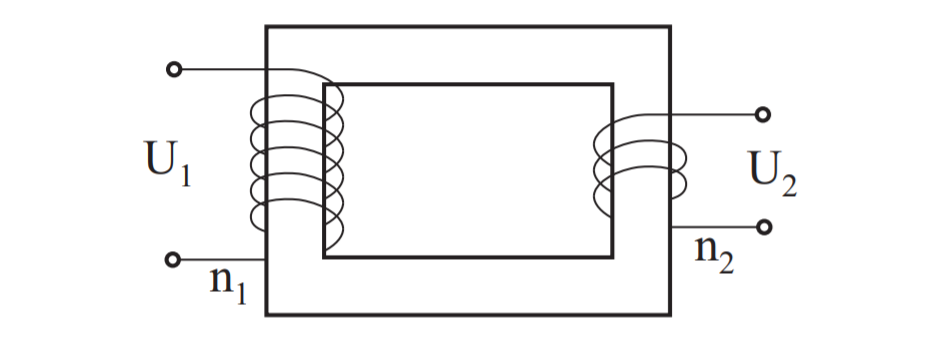
\includegraphics[scale=0.4]{transformator.png}
%~
%}
%\end{figure}



\section{Geräteliste}

\begin{table}[H]
\caption{Liste der verwendeten Geräte}

~

\begin{tabular}{l|p{3cm}p{3.5cm}llll}
Abk. & Gerätename    & Hersteller & Modell  \\
\hline
S & Spektralphotometer & THOR-Labs & CCS200/M \\
L & Lampe & THOR-Labs & QTH10/M \\
FR & Filter Rot & \\
FB & Filter Blau & \\
KW & Küvette mit Wasser &\\
KM & Küvette mit Methylenblau \\
GP & Glasplatte
\end{tabular}
\end{table}





\section{Beschreibung der Versuchsanordnung}

\section{Versuchsdurchführung und Messwerte}

Als erstes wurde die Halogen-Lampe eingeschalten und die Spektralphotometer-Software SPLICCO gestartet. In der Software wurde dann der Wellenlängenbereich auf $400-800$~nm eingestellt, die Integrationszeit (integration time) auf $0.5-2.0$~ms (genauen Wert hier nach Durchführung einfügen) eingestellt, sodass das Spektrum der Lichtquelle über den gesamten angezeigten y-Achsenabschnitt gut skaliert wird. Die durchschnittlichen Aufnahmen (average scans) auf 50 eingestellt.
Zur Korrektur der Hintergrundbeleuchtung musste die Halogen-Lampe wieder ausgeschalten werden und mit Save Background Correction gespeichert werden. So wird die Hintergrundbeleuchtung bei den folgenden Messungen automatisch abgezogen. Falls sich die Hintergrundbeleuchtung im Laufe des Experiments ändern sollte, so muss diese Korrektur wiederholt werden.


\subsection{Bestimmung der Transmission und der Extinktion für verschiedene Farbfilter}

Hierfür wurde zunächst das Intensitätsspektrum der Halogenlampe ohne Filter im Strahlengang (Referenzspektrum) aufgezeichnet und als csv.Datei exportiert.

Danach wurden die Intensitätsspektren sowohl für zwei einzelne Farbfilter also auch für beide Farbfilter gemeinsam gemessen. Auch diese Daten wurden aufgezeichnet und als csv.Dateien exportiert.

Um mögliche Messungenauigkeiten zu minimieren werden alle Spektren 5 mal aufgezeichnet und entsprechend gemittelt.

Die gemessenen Intensitäten sind in Grafik \ref{fig:I_Methyl} zusammengefasst.

\begin{figure}[H]
\centering
\caption{Zusammenhang zwischen Intensität und Wellenlänge bei gegebenen Filter.}
\label{fig:I_Methyl}
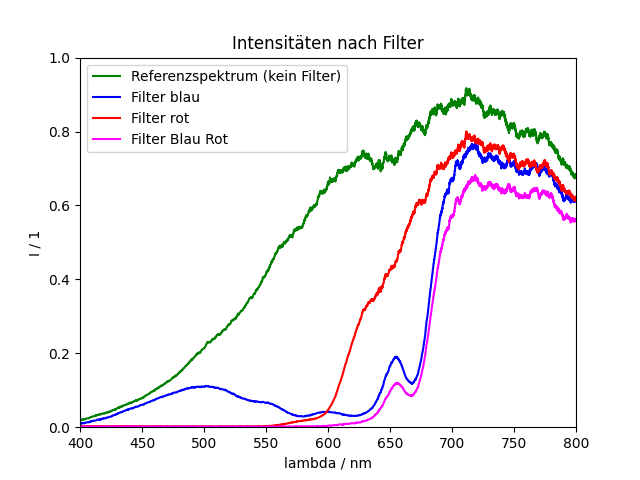
\includegraphics[scale=0.7]{Intensitaeten.png}
\end{figure}





\subsection{Bestimmung der Stoffmengenkonzentration einer Methylenblaulösung}

Dafür wurde zuerst der Filterhalter gegen den Küvettenhalter ausgetauscht und die Küvette mit Wasser im Halter platziert und das Transmissionsspektrum von Wasser als Referenz gemessen. Dann wurde die Küvette mit Wasser gegen die Küvette mit Methylenblausäure ausgetauscht und ebenfalls das Transmissionsspektrum gemessen.



\begin{figure}[H]
\centering
\caption{Zusammenhang zwischen Intensität und Wellenlänge einmal bei einer Küvette mit Wasser (grau) und einmal bei einer Küvette mit einer Lösung mit Methylenblau.}
\label{fig:I_methyl}
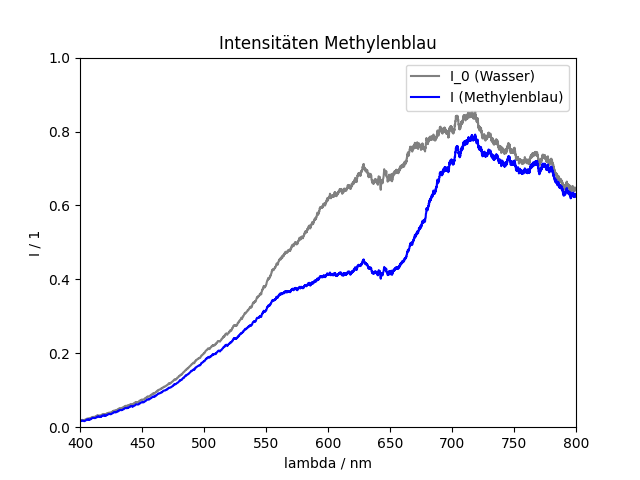
\includegraphics[scale=0.7]{Intensitaeten_Methyl.png}
\end{figure}





\subsection{Bestimmung der Dicke einer Glasplatte durch das Transmissionsspektrum}

Hierfür wurden zunächst die Farbfilter aus dem Strahlengang entfernt und wieder ein Referenzspektrum gemessen. Danach wurde die Glasplatte anstelle der Farbfilter im Strahlengang platziert und das Intensitätsspektrum mit Platte gemessen.



\begin{figure}[H]
\centering
\caption{Zusammenhang zwischen Intensität und Wellenlänge einmal mit der Glasplatte und einmal ohne Glasplatte als Referenz.}
\label{fig:I_glas}
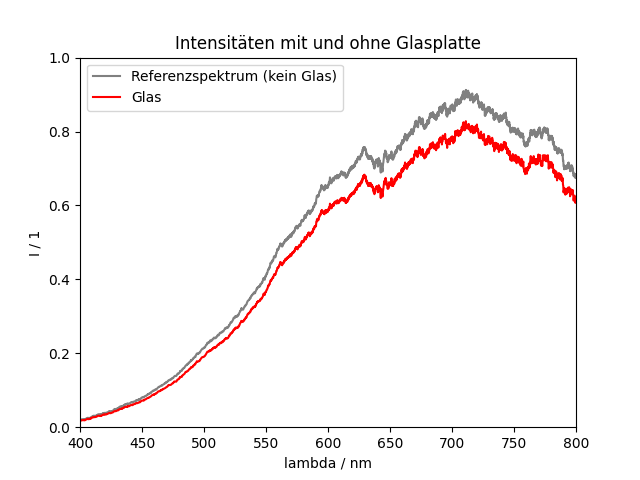
\includegraphics[scale=0.7]{Glas_Intensitaeten.png}
\end{figure}



\section{Auswertung}

\subsection{Bestimmung von Transmission und Extinktion für verschiedene Farbfilter}


\begin{figure}[H]
\centering
\caption{Zusammenhang zwischen Transmissionen und Wellenlänge bei gegebenen Filter.}
\label{fig:T_Farben}
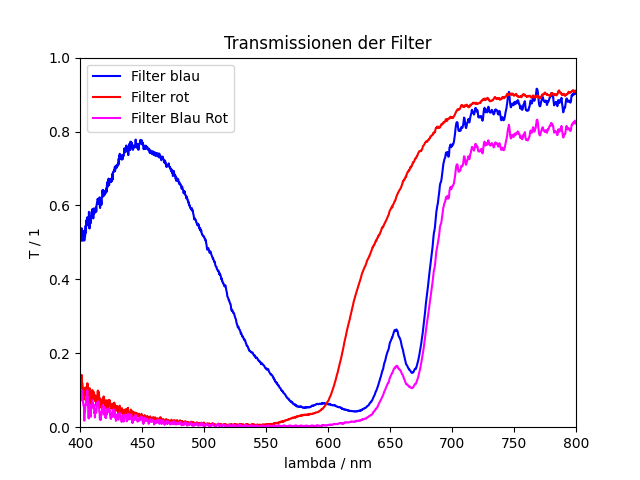
\includegraphics[scale=0.7]{Transmissionen.png}
\end{figure}



\begin{figure}[H]
\centering
\caption{Zusammenhang zwischen Extinktion und Wellenlänge bei gegebenen Filter.}
\label{fig:Ext}
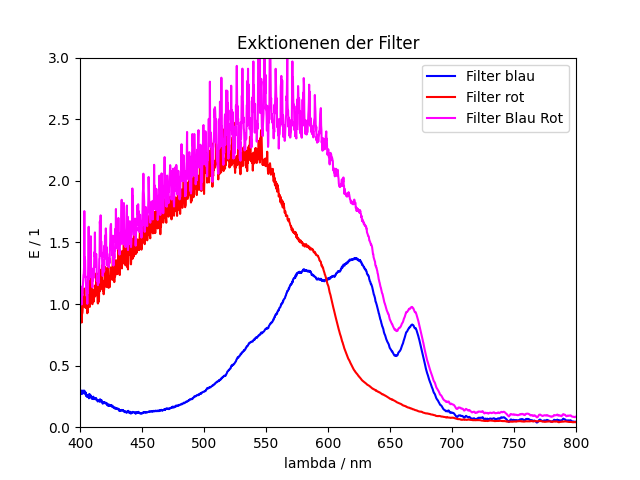
\includegraphics[scale=0.7]{Extinktionen.png}
\end{figure}

\begin{figure}[H]
\centering
\caption{Summe der Extinktionen des roten und blauen Filters (jeweils extra gemessen) hier in orange verglichen mit der gemeinsam gemessenen Extinktion hier in magenta.}
\label{fig:sum_ext}
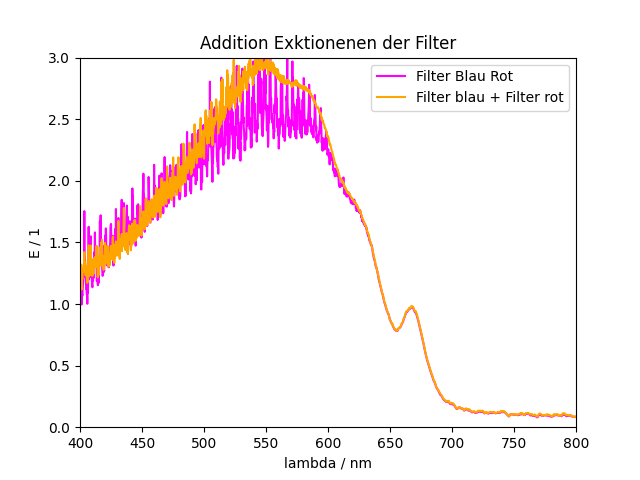
\includegraphics[scale=0.7]{Extinktionen_addition.png}
\end{figure}


\begin{figure}[H]
\centering
\caption{Intensitäten bei Vertauschung der Reihenfolge der Filter. Es ist kaum ein Unterschied zu erkennen. Daher ist in Grafik \ref{fig:reihenfolge2} die Differenz dargestellt.}
\label{fig:reihenfolge1}

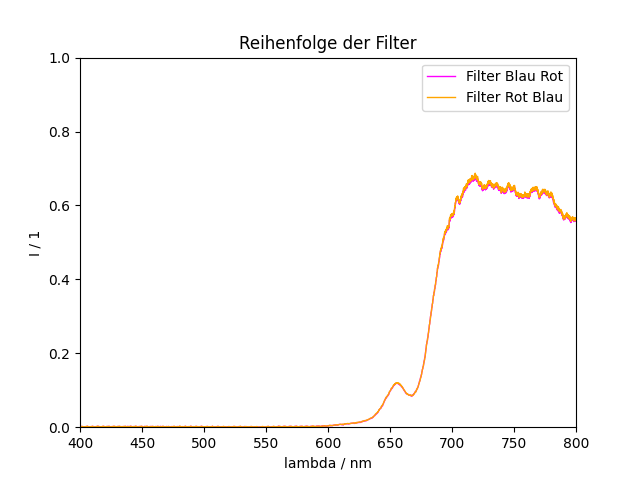
\includegraphics[scale=0.7]{reihenfolge1.png}
\end{figure}



\begin{figure}[H]
\centering
\caption{Differenz der Intensitäten bei Vertauschung der Reihenfolge der Filter. Man kann hier eine Unsicherheit für die Auswertung ablesen.}
\label{fig:reihenfolge2}

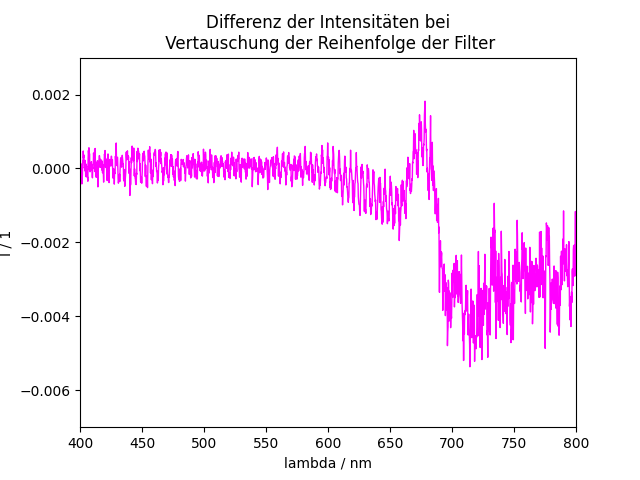
\includegraphics[scale=0.7]{reihenfolge2.png}
\end{figure}






\subsection{Bestimmung der Stoffmengenkonzentration einer Methylenblaulösung}

Grafik~\ref{fig:Trans_Ex_Methyl} zeigt die Transmission und Extinktion der Lösung mit Methylenblau.

Zur Berechnung der Konzentration benötigt man Formel~\eqref{eq:konzentration}. Durch Umformungen, Regeln für Logarithmen und Fehlerrechnung erhält man
\begin{align*}
c = \frac{\log(I_0) - \log(I_T)}{\varepsilon\cdot d} \pm \left(\frac{\dfrac{\Delta I_0}{I_0} + \dfrac{\Delta I_T}{I_T}}{\varepsilon\cdot d} + \frac{\log(I_0) - \log(I_T)}{\varepsilon\cdot d^2} \cdot \Delta d\right)
\end{align*}

Gemäß \cite{moodle} können wir den  dekadischer Extinktionskoeffizienten von Methylenblau bei einer Wellenlänge von 664~nm bei
\begin{align*}
\varepsilon =  77790~\frac{\text{Liter}}{\text{mol~cm}}
\end{align*}
annehmen. Die Schichtdicke der Lösung in der Küvette beträgt außerdem 1~cm mit der angenommenen Unsicherheit von $10~\mu$m. Insgesamt ergibt sich 
\begin{align*}
c = (2.46 \pm 0.09)\cdot 10^6~\text{mol/Liter} 
\end{align*}

wobei die Werte für $I_0$ und $I_T$ mit Hilfe eines Python Skriptes gemittelt wurden.

\begin{figure}[H]
\centering
\caption{Transmission und Extinktion der Lösung mit Ethylenblau.}
\label{fig:Trans_Ex_Methyl}
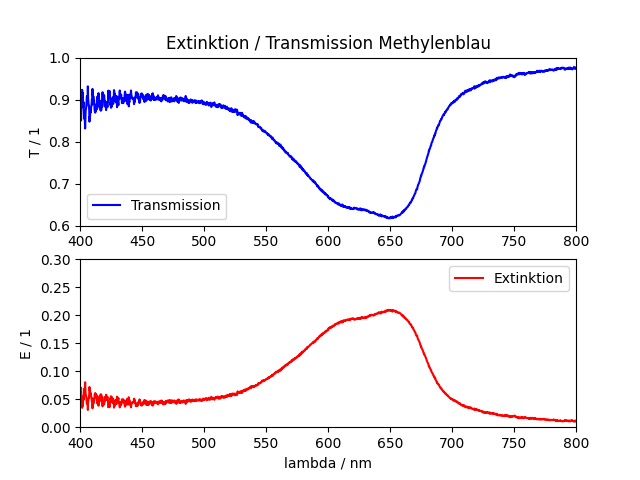
\includegraphics[scale=0.7]{Transmission_Extinktion_Methyl.png}

\end{figure}




\subsection{Bestimmung der Dicke einer Glasplatte durch das Transmissionsspektrum}

Das Maximum aus Grafik~\ref{fig:I_glas} ist gegeben durch
\begin{align*}
I_{\text{max}} = 0.83\qquad \text{bei} \qquad \lambda = 711.15 
\end{align*}

Entsprechend wird in Grafik~\ref{fig:T_glas} die Skalierung gewählt. Dort werden die Maxima der Transmission abgelesen. Diese sind in Tabelle~\ref{tab:trans_max_glas} zusammengefasst.

\begin{table}[H]
\centering
\caption{Transmissionsmaxima im Bereich $\lambda_m\in[700,720]~$nm. $m$ Begungsordnung, $\nu_m$ Wellenzahl, $T_m$ Wert der Transmission}
\label{tab:trans_max_glas}
\begin{tabular}{cccc}
m & $\lambda_m$ / nm & $\nu_m$ / $\mu$m${}^{-1}$ & T / 1 \\
\hline1 & 700.6 & 1.427 & 0.904\\
2 & 701.7 & 1.425 & 0.908\\
3 & 702.7 & 1.423 & 0.911\\
4 & 703.8 & 1.421 & 0.909\\
5 & 704.8 & 1.419 & 0.908\\
6 & 706.0 & 1.417 & 0.907\\
7 & 706.9 & 1.415 & 0.906\\
8 & 708.1 & 1.412 & 0.908\\
9 & 709.0 & 1.410 & 0.909\\
10 & 710.2 & 1.408 & 0.910\\
11 & 711.4 & 1.406 & 0.908\\
12 & 712.3 & 1.404 & 0.909\\
13 & 713.5 & 1.402 & 0.907\\
14 & 714.4 & 1.400 & 0.910\\
15 & 715.6 & 1.397 & 0.910\\
16 & 716.8 & 1.395 & 0.909\\
17 & 717.8 & 1.393 & 0.909\\
18 & 718.9 & 1.391 & 0.910\\
\end{tabular}

\end{table}

Aus \cite{moodle} geht hervor, dass die Brechzahl bei Glas $n_p = 1.519$ ist, wenn $\lambda=700~$nm. Wir nehmen zusätzlich $\Delta n_p = 0.001$ an.
Zusätzlich besteht laut \cite{moodle} ein linearer Zusammenhang 
\begin{align*}
\nu_M = k\cdot m
\end{align*}
Durch Lineare Regression lässt sich dieses $k$ Zusammenhang berechnen. Zusätzlich gilt
\begin{align*}
k = \frac{1}{2\cdot n_p\cdot d}
\end{align*}
wobei $d$ unsere gesuchte Dicke ist. Durch Berechnung der Regression ergibt sich
\begin{align*}
k = (-2.14 \pm 0.08)\cdot 10^{-6}~\text{nm}^{-1} 
\end{align*}

und daraus folgt
\begin{align*}
d = \frac{1}{2\cdot n_p\cdot k} \pm \left( \frac{\Delta n_p}{2\cdot n_p^2\cdot k} + \frac{\Delta k}{2\cdot n_p\cdot k^2}\right)
\end{align*}
Die Dicke der Glasplatte beträgt letztendlich
\begin{align*}
d = (0.15 \pm 0.01)~\text{mm} 
\end{align*}


\begin{figure}[H]
\centering
\caption{Transmission und Extinktion bei Untersuchung der Glasplatte. Die Maxima der Transmission sind mit einer vertikalen Linie gekennzeichnet.}
\label{fig:T_glas}
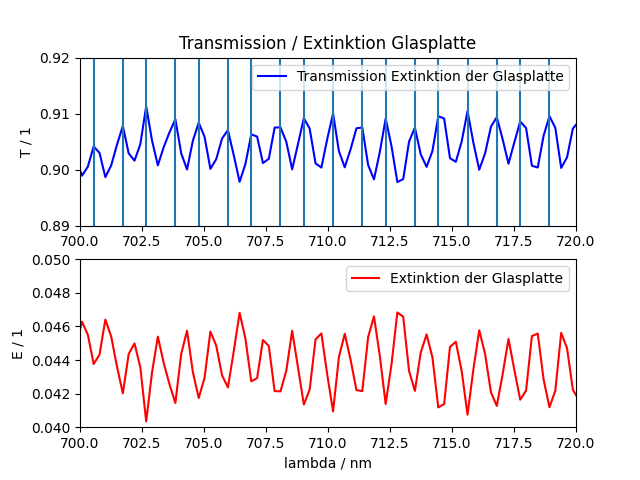
\includegraphics[scale=0.7]{Glas_Transmission_Extinktion.png}
\end{figure}





\section{Diskussion}

Man kann in den aufgenommenen Spektren ein starkes Rauschen erkennen. Dies kann sich einerseits durch die Änderung von Lichtverhältnissen im Raum ergeben, andererseits durch leichte Unreiheiten auf den Linsen und Oberflächen der optischen Geräte.

Die Reihenfolge der Farbfilter spielt eine untergeordnete Rolle. In Grafiken \ref{fig:reihenfolge1} und \ref{fig:reihenfolge2} kann man sehen, dass die Intensitäten sehr wenige Abweichungen haben.

Die Additivität von Extinktionen lässt sich auch mathematisch begründen. Sei $I_0$ die Intensität zu Beginn, $I_1$ nach Durchgang durch Filter 1 und $I_2$ die Intensität nach Durchgang durch Filter 2, dann gilt
\begin{align*}
E_1 + E_2 = \log\left(\frac{I_0}{I_1}\right) + \log\left(\frac{I_1}{I_2}\right) = \log\left(\frac{I_0}{I_1}\cdot \frac{I_1}{I_2}\right) = \log\left(\frac{I_0}{I_2}\right) = E_{1,2}
\end{align*}



Für die Glasplatte wurde leider kein allgemeiner Wert gefunden, den man zur Verwendung heranziehen könnte.




\section{Zusammenfassung}






\begin{thebibliography}{9}
\bibitem{moodle} Unterlagen aus Moodle, J. Krenn, G. Paltauf, bereitgestellt von der KF Universität Graz.
\end{thebibliography}


%\newpage 
%\appendix
%\section{Python Skript}



\definecolor{commentgreen}{RGB}{2,112,10}
\definecolor{eminence}{RGB}{108,48,130}
\definecolor{weborange}{RGB}{255,165,0}
\definecolor{frenchplum}{RGB}{129,20,83}

\lstdefinelanguage{python}{
    morekeywords={def, for, range, abs, return},
    otherkeywords={<-,->, |>, \%\{, \}, \{, \, (, )},
    sensitive=true,
    morecomment=[l]{\#},
    morecomment=[n]{/*}{*/},
    morecomment=[s][\color{purple}]{:}{\ },
    morestring=[s][\color{orange}]"",
    commentstyle=\color{commentgreen},
    keywordstyle=\color{eminence},
    stringstyle=\color{red},
	basicstyle=\ttfamily,
	breaklines,
	showstringspaces=false,
	frame=tb
}
\lstset{
extendedchars=\true,
inputencoding=utf8
}

%\lstinputlisting[language=Python,captionpos=b, label=lst:test,caption={Python Skript}]{plot.py}

%\lstinputlisting[language=Python,captionpos=b, label=lst:test,caption={Bessel Auswertung}]{generate_numbers_bessel.py}


%\lstinputlisting[language=Python,captionpos=b, label=lst:test,caption={Zerstreuungslinse Auswertung}]{generate_numbers_zerstreuungslinse.py}


\end{document}
